%!TEX root = ../../../_main.tex
\subsection{Bruhat ordering}
\label{sec:coxeter-groups-bruhat-ordering}

We now investigate ways to partially order the elements of a Coxeter group. Futhermore, this ordering should be compatible with the length function, i.e. for $w,v \in W$ we have $l(w) < l(v)$ whenever $w \leq v$.

\begin{defi}
	\typedlabel{defi:poset}
	Let $M$ be a set. A binary relation $\leq$ is called a \defword{partial order} over $M$, if for all $a,b,c \in M$ it satisfies the conditions
	\begin{enumerate}
		\item $a \leq a$ (\defword{reflexivity}),
		\item $a \leq b \wedge b \leq a \Rightarrow a=b$ (\defword{antisymmetry}) and
		\item $a \leq b \wedge b \leq c \Rightarrow a \leq c$ (\defword{transitivity}).
	\end{enumerate}
	In this case $(M,\leq)$ is called a \defword{poset}. If two elements $a \leq b \in M$ are immediate neighbors, i.e. there is no third element $c \in M$ with $a \leq c \leq b$ we say that $b$ \defword{covers} $a$. A poset is called \defword{graded poset} if there is a map $\rho : M \to \nn$ so that $\rho(b) - 1 = \rho(a)$ whenever $b$ covers $a$. In this case $\rho$ is called the \defword{rank function} of the graded poset.
\end{defi}

\begin{defi}
	\typedlabel{defi:hasse-diagram}
	Let $(M,\leq)$ be a poset. The \defword{Hasse diagram} of the poset is the graph obtained in the following way: Add a vertex for each element in $M$. Then add a directed edge from vertex $a$ to $b$ whenever $b$ covers $a$.
\end{defi}

\begin{exam}
	Suppose we have an arbitrary set $M$. Then the powerset $\mathcal P (M)$ can be partially ordered by the subset relation, so $(\mathcal P (M), \subseteq)$ is a poset. Indeed this poset is always graded with the cardinality function as rank function. In Figure \ref{fig:poset-xyz-subsets} we see the Hasse diagram of this poset with $M = \{x,y,z\}$.

	\begin{figure}[ht]
		\centering
		%!TEX root = ../../_main.tex
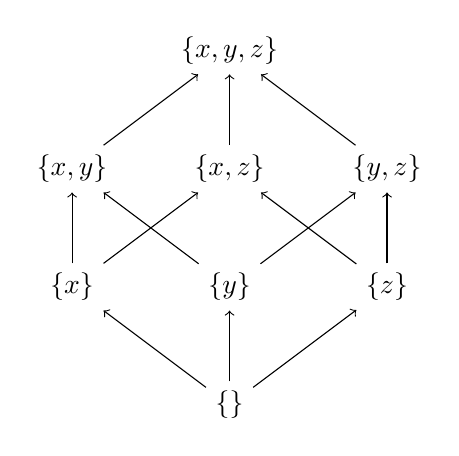
\begin{tikzpicture}
	\tikzstyle{every node}=[]
	\tikzstyle{relation}=[->]

	\node (xyz) at (0,0) {$\{x,y,z\}$};
	\node (xy) at (-2,-1.5) {$\{x,y\}$};
	\node (xz) at (0,-1.5) {$\{x,z\}$};
	\node (yz) at (2,-1.5) {$\{y,z\}$};
	\node (x) at (-2,-3) {$\{x\}$};
	\node (y) at (0,-3) {$\{y\}$};
	\node (z) at (2,-3) {$\{z\}$};
	\node (0) at (0,-4.5) {$\{\}$};
	\draw[relation] (0) -- (x);
	\draw[relation] (0) -- (y);
	\draw[relation] (0) -- (z);
	\draw[relation] (x) -- (xy);
	\draw[relation] (x) -- (xz);
	\draw[relation] (y) -- (xy);
	\draw[relation] (y) -- (yz);
	\draw[relation] (z) -- (xz);
	\draw[relation] (z) -- (yz);
	\draw[relation] (xy) -- (xyz);
	\draw[relation] (xz) -- (xyz);
	\draw[relation] (yz) -- (xyz);
\end{tikzpicture}
		\caption{Hasse diagram of the set of all subsets of $\{x,y,z\}$ order by the subset relation}
		\label{fig:poset-xyz-subsets}
	\end{figure}
\end{exam}

\begin{defi}
	\typedlabel{defi:bruhat-ordering}
	Let $(W,S)$ be a Coxeter system and $T = \cup_{w \in W} wSw^{-1}$ the set of all reflections in $W$. We write $w' \to w$ if there is a $t \in T$ with $w't = w$ and $l(w') < l(w)$. If there is a sequence $w' = w_0 \to w_1 \to \ldots \to w_m = w$ we say $w' < w$. The resulting relation $w' \leq w$ is called \defword{Bruhat ordering}, denoted by $\Br(W)$.
\end{defi}

\begin{lemm}
	\typedlabel{lemm:bruhat-ordering-is-poset}
	Let $(W,S)$ be a Coxeter system. Then $\Br(W)$ is a poset.

	\begin{proof}
		The Bruhat ordering is reflexive by definition. Since the elements in sequences $e \to w_1 \to w_2 \to \ldots$ are strictly ascending in length, it must be antisymmetric. By concatenation of sequences we get the transitivity.
	\end{proof}
\end{lemm}

What we really want is the Bruhat ordering to be graded with the length function as rank function. By definition we already have $v < w$ iff $l(v) < l(w)$, but its not that obvious that two immediately adjacent elements differ in length by exactly 1. Beforehand let us just mention two other partial orderings, where this property is obvious by definition:

\begin{defi}
	Let $(W,S)$ be a Coxeter system. The ordering $\leq_R$ defined by $u \leq_R w$ iff $uv = w$ for some $u \in W$ with $l(u) + l(v) = l(w)$ is called the \defword{right weak ordering}. The left-sided version $u \leq_L w$ iff $vu = w$ is called the \defword{left weak ordering}.
\end{defi}

To ensure the Bruhat ordering is graded as well, we need another characterization of the Bruhat ordering in terms of subexpressions.

\begin{prop}
	\typedlabel{prop:u-leq-w-then-us-leq-w-or-us-leq-ws}
	\theocite{Proposition 5.9}{humphreys:coxeter}
	Let $(W,S)$ be a Coxeter system, $u,w \in W$ with $u \leq w$ and $s \in S$. Then $us \leq w$ or $us \leq ws$ or both.

	\begin{proof}
		We can reduce the proof (\todo why?) to the case $u \to w$, i.e. $ut = w$ for a $t \in T$ with $l(v) < l(u)$. Let $s = t$. Then $us \leq w$ and we are done. In case $s \neq t$ there are two alternatives for the lengths. We can have $l(us) = l(u) - 1$ which would mean $us \to u \to w$, so $us \leq w$.

		Assume $l(us) = l(u) + 1$. For the reflection $t' = sts$ we get $(us)t' = ussts = uts = ws$. So we have $us \leq ws$ iff $l(us) < l(ws)$. Suppose this is not the case. Since we have assumed $l(us) = l(u) + 1$ any reduced expression $u = s_1 \cdots s_r$ for $u$ yields a reduced expression $us = s_1 \cdots s_r s$ for $us$. With the \ref{theo:strong-exchange-condition} we can obtain $ws = ust'$ from $us$ by omitting one factor. This omitted factor cannot be $s$ since $s \neq t$. This means $ws = s_1 \cdots \hat s_i \cdots s_r s$ and so $ws = s_1 \cdots \hat s_i \cdots s_r$, contradicting to our assumption $l(u) < l(w)$
	\end{proof}
\end{prop}

\begin{theo}
	\typedlabel{theo:bruhat-subexpression-characterization}
	\theocite{Theorem 5.10}{humphreys:coxeter}
	Let $(W,S)$ be a Coxeter system and $w \in W$ with any reduced expression $w = s_1 \cdots s_r$ and $s_i \in S$. Then $u \leq w$ (in the Bruhat ordering) iff $u$ can be obtained as a subexpression of this reduced expression.

	\begin{proof}
		\todo
	\end{proof}
\end{theo}

This characterization of the Bruhat ordering is very handy. With it and the following short lemma we will be in the position to show that $\Br(W)$ is graded with rank function $l$.

\begin{lemm}
	\typedlabel{lemm:dont-know}
	\theocite{Lemma 5.11}{humphreys:coxeter}
	Let $(W,S)$ be a Coxeter system, $u,w \in W$ with $u < w$ and $l(w) = l(u) + 1$. In case there is a generator $s \in S$ with $u < us$ but $us \neq w$, then both $w < ws$ and $us < ws$.

	\begin{proof}
		Due to \ref{prop:u-leq-w-then-us-leq-w-or-us-leq-ws} we have $us \leq w$ or $us \leq ws$. Since $l(us) = l(w)$ and $us \neq w$ the first case is impossible. So $us \leq ws$ and because of $u \neq w$ already $us < ws$. In turn, $l(w) = l(us) < l(ws)$, forcing $w < ws$.
	\end{proof}
\end{lemm}

\begin{prop}
	\typedlabel{prop:bruhat-intervals}
	\theocite{Proposition 5.11}{humphreys:coxeter}
	Let $(W,S)$ be a Coxeter system and $u < w$. Then there are elements $w_0,\ldots,w_m \in W$ such that $u = w_0 < w_1 < \ldots < w_m = w$ with $l(w_i) = l(w_{i-1}) + 1$ for $1 \leq i \leq m$.

	\begin{proof}
		We induce on $r = l(u) + l(w)$. In case $r = 1$ we have $u = e$ and $w = s$ for an $s \in S$ and are done. Conversely suppose $r > 1$. Then there is a reduced expression $w = s_1 \cdots s_r$ for $w$. Lets fix this expression. Then $l(w s_r) < l(w)$. Thanks to \ref{theo:bruhat-subexpression-characterization} there must be a subexpression of $w$ with $u = s_{i_1} \cdots s_{i_q}$ for some $i_1 < \ldots < i_q$. We distinguish between two cases:

		\begin{description}
			\item[$u < us$:] If $i_q = r$, then $us = s_{i_1} \cdots s_{i_q} s = s_{i_1} \cdots s_{i_{q-1}}$ which is also a subexpression of $ws$. This yields $u < us \leq ws < w$. Since $l(ws) < r$ there is, by induction, a sequence of the desired form. The last step from $ws$ to $w$ also differs in length by exactly 1, so we are done. If $i_q < r$ then $u$ is itself already a subexpression of $ws$ and we can again find a sequence from $u$ to $ws$ strictly ascending length by 1 in each step and have one last step from $ws$ to $w$ also increasing length by 1.
			\item[$us < u$:] Then by induction we can find a sequence from $us$ to $w$, say $us = w_0 < \ldots < w_m = w$, where the lengths of neighbored elements differ by exactly 1. Since $w_0 s = u > us = w_0$ and $w_m s = ws < w = w_m$ there must be a smallest index $i \geq 1$, such that $w_i s < w_i$, which we choose. Suppose $w_i \neq w_{i-1} s$. We have $w_{i-1} < w_{i-1}s \neq w_i$ and due to \ref{lemm:dont-know} we get $w_i < w_i s$. This contradicts to the minimality of $i$. So $w_i = w_{i-1} s$. For all $1 \leq j < i$ we have $w_j \neq w_{j-1} s$, because of $w_j < w_j s$. Again we apply \ref{lemm:dont-know} to receive $w_{j-1} s < w_j s$. Alltogether we can construct a sequence
			$$ u = w_0 s < w_1 s < \ldots < w_{i-1} s = w_i < w_{i+1} < \ldots w_m = w, $$
			which matches our assumption. \qedhere
		\end{description}
	\end{proof}
\end{prop}

\begin{coro}
	\typedlabel{coro:bruhat-ordering-is-graded}
	Let $(W,S)$ be a Coxeter system and $\Br(W)$ the Bruhat ordering poset of $W$. Then $\Br(W)$ is graded with $l:W \to \nn$ as rank function.

	\begin{proof}
		Let $u,w \in W$ with $w$ covering $u$. Then \ref{prop:bruhat-intervals} says there is a sequence $u = w_0 < \ldots < w_m = w$ with $l(w_i) = l(w_{i-1}) + 1$ for $1 \leq i \leq m$. Since $w$ covers $u$ it must be $m = 1$ and so $u < w$ with $l(w) = l(u) + 1$.
	\end{proof}
\end{coro}

\begin{theo}[Lifting Property]
	\namedlabel{theo:lifting-property}
	\theocite{Theorem 1.1}{deodhar:bruhat-order}
	Let $(W,S)$ be a Coxeter system and $v,w \in W$ with $v \leq w$. Suppose $s \in S$ with $s \in D_R(w)$. Then
	\begin{enumerate}
		\item $vs \leq w$,
		\item $s \in D_R(v) \Rightarrow vs \leq ws$.
	\end{enumerate}

	\begin{proof}
		We use the alternative subexpression characterization of the Bruhat ordering from \ref{theo:bruhat-subexpression-characterization}.
		\begin{enumerate}
			\item Since $s \in D_R(w)$ there exists a reduced expression $w = s_1 \cdots s_r$ with $s_r = s$. Due to $v \leq w$ we can obtain $v$ as a subexpression $v = s_{i_1} \cdots s_{i_q}$ from $w$. If $i_q = r$ then $vs = s_{i_1} \cdots s_{i_q} s = s_{i_1} \cdots s_{i_{q - 1}}$ is also a subexpression of $w$. Else, if $i_q \neq r$ then $v$ is a subexpression of $ws = s_1 \cdots s_{r-1}$ and so $vs$ is again a subexpression of $w = s_1 \cdots s_{r-1} s$. In both cases we get $vs \leq w$.
			\item If we additionally assume $s \in D_R(v)$ then we can always find a reduced expression $w = s_1 \cdots s_r$ with $s_r = s$ having $u = s_{i_1} \cdots s_{i_q}$ as subexpression with $s_{i_q} = s$. This yields $vs = s_{i_1} \cdots s_{i_{q-1}} \leq s_1 \cdots s_{r-1} = ws$. \qedhere
		\end{enumerate}
	\end{proof}
\end{theo}

The \ref{theo:lifting-property} seems quite innocent, but when trying to investigate facts around the Bruhat ordering it prooves to be one of the key tools in many cases.